% !TEX root = ../main.tex

\begin{frame}{Hardware Camera Controls Panasonic}
	\begin{columns}[T,onlytextwidth]
		\column{0.5\textwidth}
	\begin{figure}
		\centering
		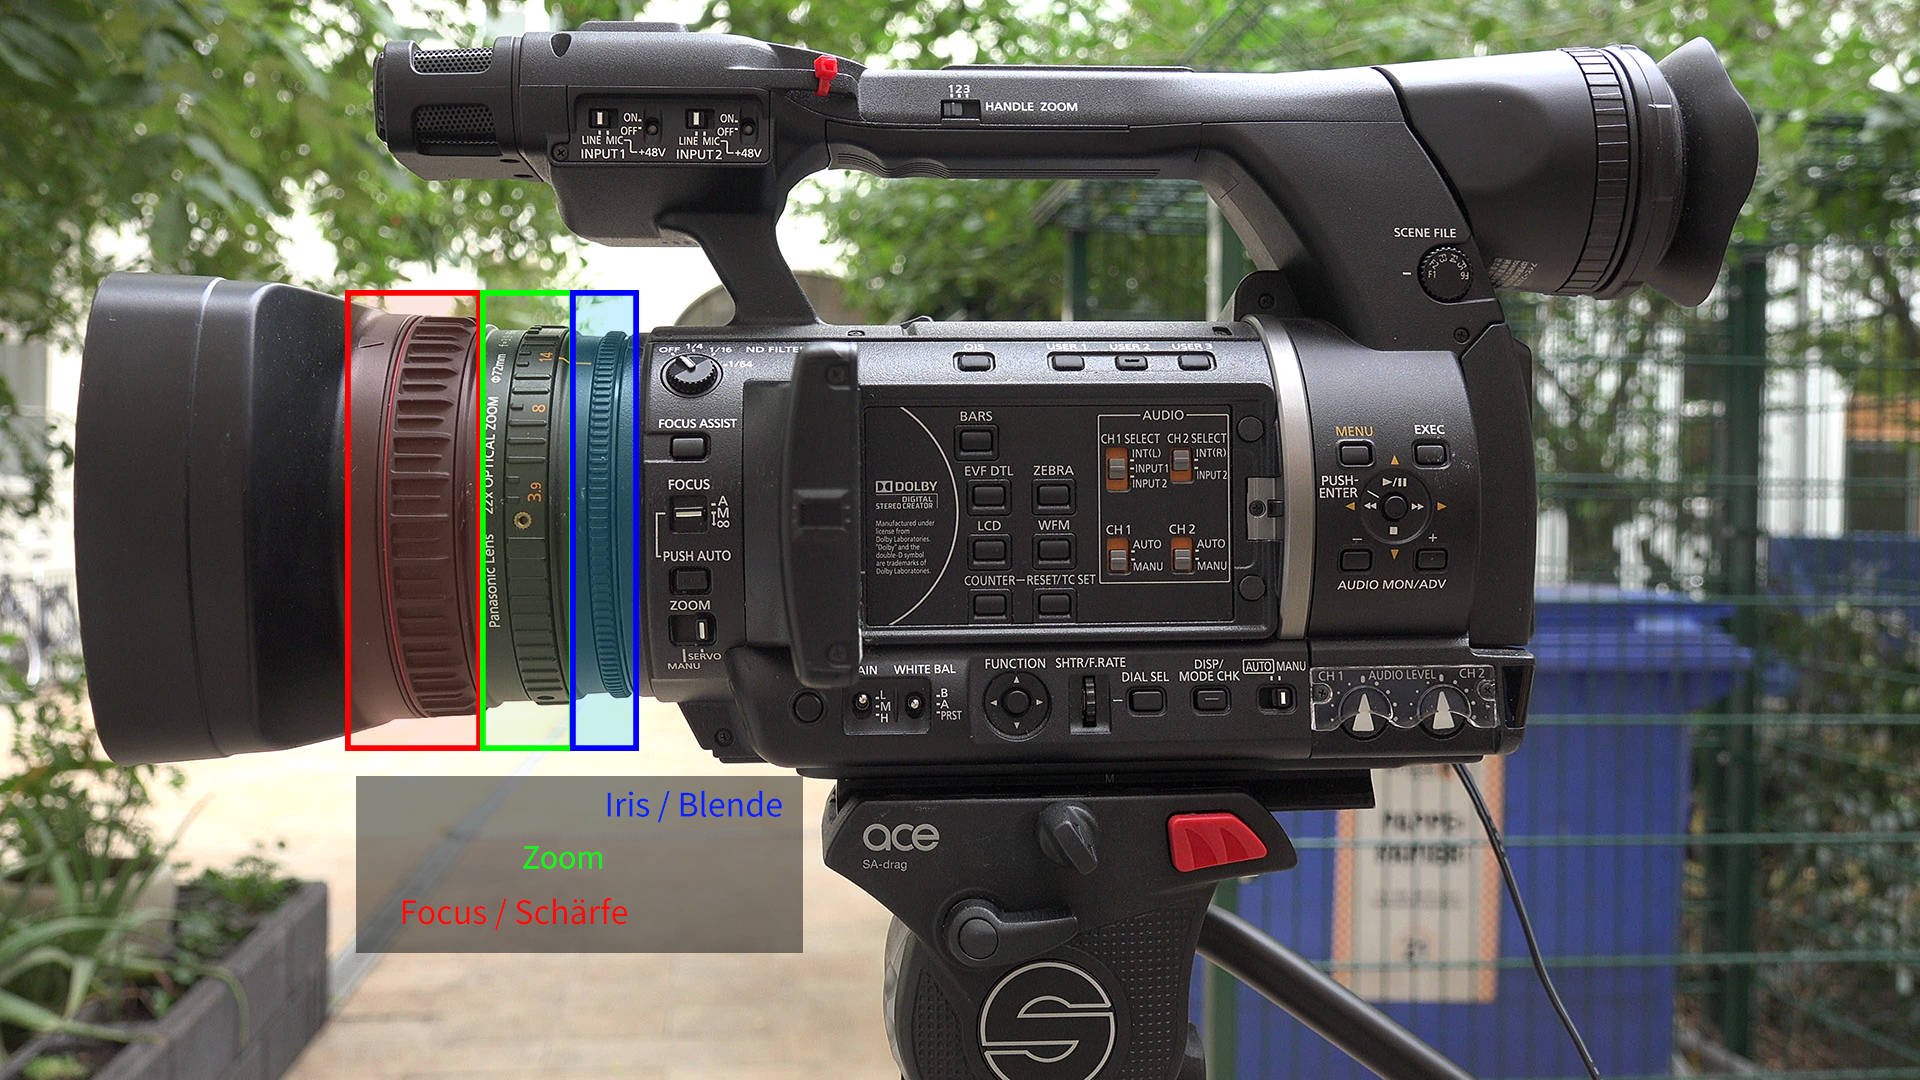
\includegraphics[width=0.9\textwidth]{images/panasonic-side-annotated.jpg}
		\caption{Panasonic Cam}
	\end{figure}
		\column{0.5\textwidth}
		Cameras are in manual mode because of difficult lighting situation.
		\begin{description}
			\item[Left Ring/red] Focus - control sharpness of the image.
			\item[Middle Ring/green] Zoom - vary the focal length.
			\item[Right Ring/blue] Iris - will have to be adjusted throughout the day. If there is anything wrong, contact C3VOC helpdesk.
		\end{description}
	\end{columns}
\end{frame}

\begin{frame}{Zoom Control Panasonic}
	\begin{columns}[T,onlytextwidth]
		\column{0.5\textwidth}
	\begin{figure}
		\centering
		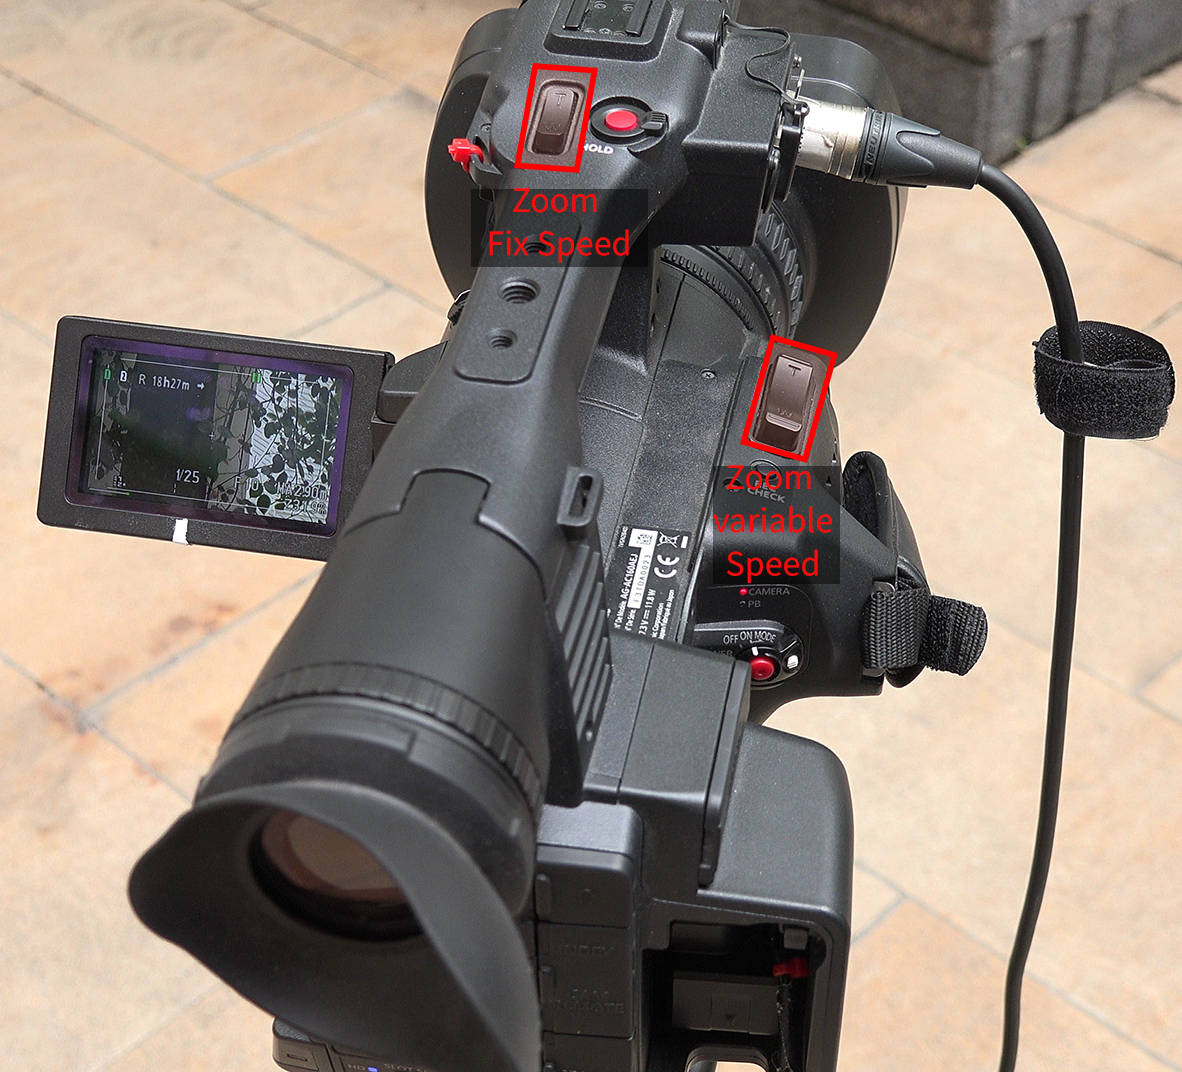
\includegraphics[width=0.99\textwidth]{images/panasonic-zoom-annotated.jpg}
		\caption{Panasonic Cam}
	\end{figure}
		\column{0.5\textwidth}
		\begin{itemize}
			\item For smooth zoom use the zoom buttons.
			\item Gentle touch $\Rightarrow$ slow zoom
			\item Top Buttons fixed speed
		\end{itemize}
	\end{columns}
\end{frame}

\begin{frame}{Display Indicators Panasonic}
	\begin{columns}[T,onlytextwidth]
		\column{0.5\textwidth}
	\begin{figure}
		\centering
		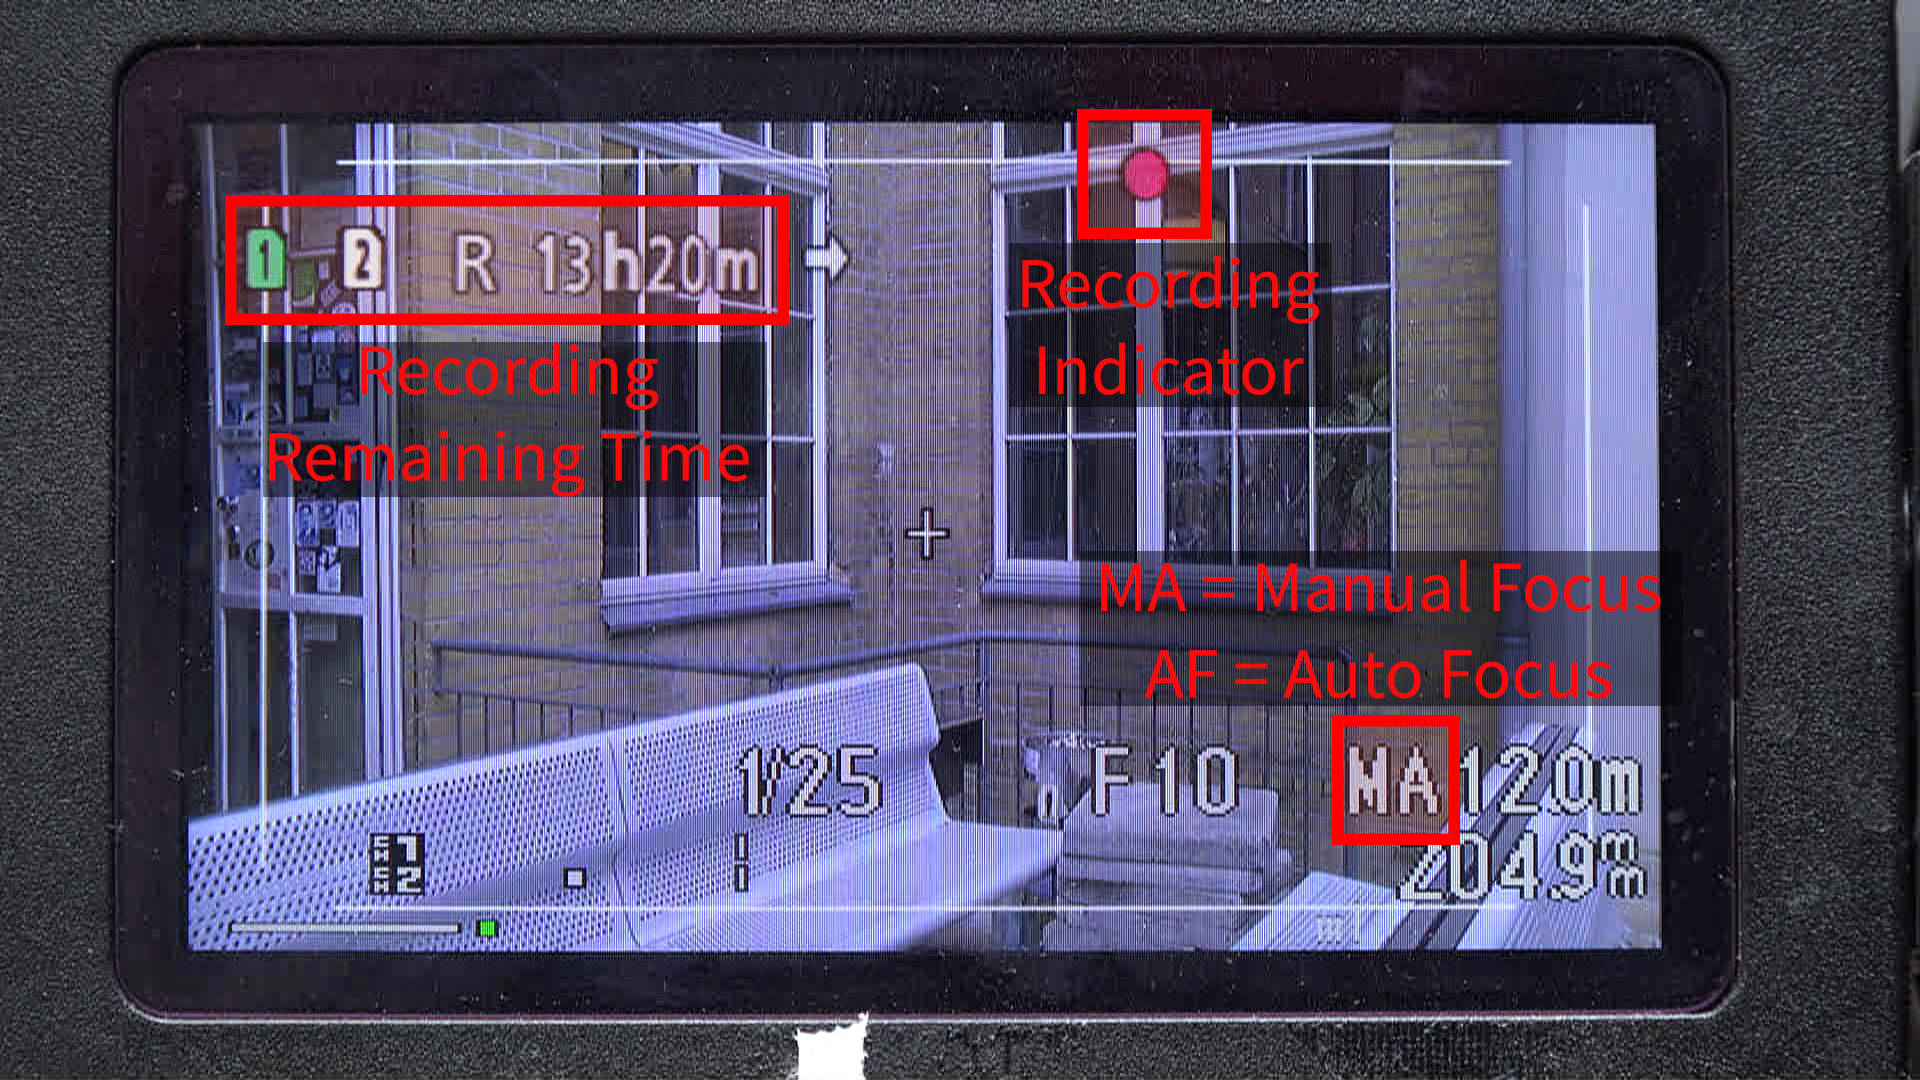
\includegraphics[width=0.9\textwidth]{images/panasonic-display-annotated.jpg}
		\caption{Panasonic Display Indicators}
	\end{figure}
		\column{0.5\textwidth}
		\begin{description}
			\item[Rec Indicator] The recording must always run, even during the break.
			\item[Focal Indicator] Use only manual focus!
			\item[Remaining Time] It must have enough remaing time before talk.
		\end{description}
		\metroset{block=fill}
		\begin{alertblock}{Alert}
			Alert the A/V-Technician if something's wrong.
		\end{alertblock}
	\end{columns}
\end{frame}
